\subsubsection{隔离策略}
FaaS系统中,资源隔离是必须的。
从资源利用的角度来说,需要隔离不同的函数运行实例,
使其相互之间不受影响,例如AWS运行Lambda最小的实例内存为128Mb,
而典型的宿主机实例则大至384Gb内存。
另一方面,从安全的角度来说,
用户代码是不可信代码,
如何防止攻击、保证底层系统安全,
也需要对函数运行进行隔离。

常规的Docker实现依赖Linux内核提供的groups、namespaces等机制实现隔离,
AWS基于Firecracker/microVM实现了自己的多层安全策略,
在性能/安全之间进行了较好的平衡,
如\cref{firecracker_isolation_model}所示\cite{Agache2020, aws_2020_function_isolation}。
这种模式的一个附加的好处是,
可以更灵活地进行监控。

\begin{figure}[ht!]
    \centering
    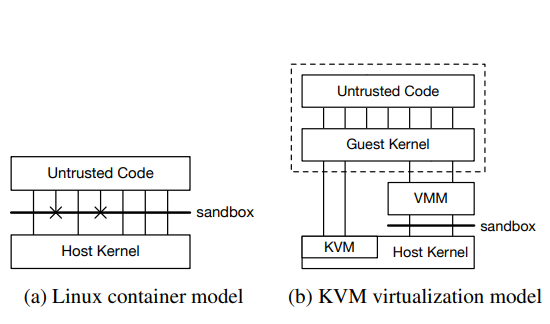
\includegraphics[width=0.7\linewidth]{images/firecrack-isolation.png}
    \caption{Docker与Firecracker的隔离方式对比\cite{Agache2020}}
    \label{firecracker_isolation_model}
\end{figure}

一些Serverless平台即支持FaaS,
也支持CaaS,
这两种模式的最终运行方式有所区别,
因此有将这两种模式的运行时进行隔离的做法,
例如字节的FaaS平台架构就采取了不同的K8s集群运行函数负载和镜像负载,
如\cref{bytedance_faas_arch}所示。

\begin{figure}[ht!]
    \centering
    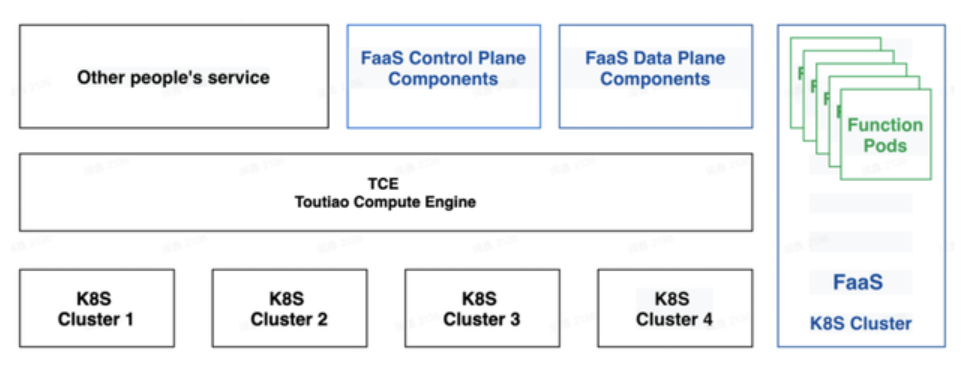
\includegraphics[width=0.7\linewidth]{images/bytedance_faas_arch.png}
    \caption{字节跳动FaaS平台架构\cite{bytedance_faas}}
    \label{bytedance_faas_arch}
\end{figure}

\subsubsection{安全容器}
由于容器技术是操作系统级的虚拟化技术,
它的安全性比虚拟机要差,
因此有一些技术用来增强容器的安全性,
也称之为安全容器技术,
例如Kata Container和Firecracker
\footnote{严格意义上Firecracker是一种轻量级虚拟技术(MicroVM)。},
以及在Kata基础上优化的RunD\cite{rund}。